% BEGIN LICENSE BLOCK
% Version: CMPL 1.1
%
% The contents of this file are subject to the Cisco-style Mozilla Public
% License Version 1.1 (the "License"); you may not use this file except
% in compliance with the License.  You may obtain a copy of the License
% at www.eclipse-clp.org/license.
% 
% Software distributed under the License is distributed on an "AS IS"
% basis, WITHOUT WARRANTY OF ANY KIND, either express or implied.  See
% the License for the specific language governing rights and limitations
% under the License. 
% 
% The Original Code is  The ECLiPSe Constraint Logic Programming System. 
% The Initial Developer of the Original Code is  Cisco Systems, Inc. 
% Portions created by the Initial Developer are
% Copyright (C) 2006 Cisco Systems, Inc.  All Rights Reserved.
% 
% Contributor(s): 
% 
% END LICENSE BLOCK
%----------------------------------------------------------------------
\chapter{Module System}
\label{modules}
\label{chapmodules}
\index{modules}
%HEVEA\cutdef[1]{section}
%----------------------------------------------------------------------

%----------------------------------------------------------------------
\section{Basics}
\subsection{Purpose of Modules}
%----------------------------------------------------------------------

The purpose of the module system is to provide a way to package
a piece of code in such a way that
\begin{itemize}
\item internals are hidden
\item it has a clearly defined interface
\item naming conflicts are avoided
\end{itemize}
In particular, this helps with
\begin{itemize}
\item Structuring of large applications:
    Modules should be used to break application programs into
    natural components and to define the interfaces between them.
\item Provision of libraries:
    All {\eclipse} libraries are modules. Their interfaces are
    defined in terms of what the module makes visible to the world.
\item Different implementations of the same predicate:
    In constraint programming it is quite common to have different
    implementations of a constraint, which all have the same declarative
    meaning but different operational behaviour (e.g.\ different amount of
    propagation, using different algorithms, exhibiting different
    performance characteristics). The module system supports that by
    allowing to specify easily which version(s) of a predicate should
    be used in a particular context.
\end{itemize}


%----------------------------------------------------------------------
\subsection{What is under Visibility Control?}
%----------------------------------------------------------------------

The {\eclipse} module system governs the visibility of the following
entities:
\begin{description}
\item[Predicate names]
    Predicates can always be used in the module where they are defined
    and optionally in other modules when they are made available.
\item[Structure names]
\index{structure}
    Structure declarations can be valid only local to a module or
    shared between several modules.
\item[Syntax settings]
\index{syntax}
    These include operator declarations
    \bipref{op/3}{../bips/kernel/syntax/op-3.html},
    syntax options and
    character classes.
    This means in particular that different modules can use different
    language dialects (e.g.\ {\eclipse} vs.\ ISO-Prolog).
\item[Container names]
\index{container}
    These include the names of record keys, nonlogical variables and references.
    They are always local to the module where they are declared.
\item[Initialization and Finalization goals]
    Modules can have initialization and finalization goals attached,
    see section \ref{initfini}.
\end{description}

Note that every definition (predicate, structure etc) is in some module,
\index{definition}
there is no space outside the modules. When you don't explicitly
specify a module, you inherit the module from the context in which
you do an operation. When you are using an interactive {\eclipse}
toplevel, a prompt will tell you in which module your input is
read and interpreted.

%----------------------------------------------------------------------
\subsection{What Modules are There?}
%----------------------------------------------------------------------

The module system is flat, i.e.\ no module is part of another module, 
and module names must be unique. There are
\begin{itemize}
\item a few basic modules that are part of the {\eclipse} runtime
    \index{runtime system}
	system and are always there. The most important one is
	called {\tt eclipse_language} and is by default imported
	into all other modules.
\item the library modules: every library consists of at least one
    \index{libraries}
	module. By convention, that module name is the library name
	and same as the base part of the library filename.
\item the application-defined modules: these are created by the
	application programmer.
\item in an interactive {\eclipse} toplevel there is one module
    \index{toplevel module}
	in which queries entered by the user are read and executed.
	That module name is displayed in a prompt.
\end{itemize}


%----------------------------------------------------------------------
\section{Getting Started}
\subsection{Creating a Module}
%----------------------------------------------------------------------

You create a module simply by starting your program code with a
\bipref{module/1}{../bips/kernel/modules/module-1.html}
directive.  This should usually be placed at the beginning of the source file
and looks like
\begin{quote}\begin{verbatim}
:- module(mymodule).
\end{verbatim}\end{quote}
As a rule, the module name should be chosen to be the same as the
file's base name (the filename without directory/folder and
suffix/extension part). E.g.\ the module {\tt mymodule} might be
contained in a file {\tt mymodule.ecl}.

Anything you define in your module is by default {\bf local} to that module.


%----------------------------------------------------------------------
\subsection{Exporting}
\index{exporting}
%----------------------------------------------------------------------

A definition is made available to the outside world by {\bf exporting} it.
All the exports of a module together form the module's {\bf interface}.
Exporting is done with the
\bipref{export/1}{../bips/kernel/modules/export-1.html}
directive, which can take
different forms depending on the kind of the exported item.

Predicates are exported as follows:
\begin{quote}\begin{verbatim}
:- export p/2.

p(X,Y) :-
        ...
\end{verbatim}\end{quote}

Structures are exported by defining them with an
\bipref{export/1}{../bips/kernel/modules/export-1.html}
instead of a
\bipref{local/1}{../bips/kernel/modules/local-1.html}
directive, e.g.
\begin{quote}\begin{verbatim}
:- export struct(book(author,title,publisher)).
\end{verbatim}\end{quote}

And the same holds for operators and other syntax settings:
\begin{quote}\begin{verbatim}
:- export op(500, xfx, before).
:- export chtab(0'$, lower_case).
:- export syntax_option(no_array_subscripts).
:- export macro(pretty/1, tr_pretty/2, []).
\end{verbatim}\end{quote}
All these declarations are valid locally in the module where they appear
{\em and} in every module that imports them.

Initialization goals are exported as follows:
\begin{quote}\begin{verbatim}
:- export initialization(writeln("I have been imported")).
\end{verbatim}\end{quote}
Unlike the other declarations above, an exported
\bipref{initialization/1}{../bips/kernel/modules/export-1.html} directive is {\em not} executed locally in
they module where it appears, but {\em only} in the context of the
module where it gets imported\footnote{
    for local initialization use :- local initialization(...).}.


%----------------------------------------------------------------------
\subsection{Importing}
\index{importing}
%----------------------------------------------------------------------

In order to use a definition that has been exported elsewhere, it has
to be {\bf imported}.  Often it is desirable to import another module's
interface as a whole, i.e.\ everything it exports.
This is achieved by an
\bipref{import/1}{../bips/kernel/modules/import-1.html}
directive of the form
\begin{quote}\begin{verbatim}
:- import amodule.
\end{verbatim}\end{quote}
If the module is in a file and has to be compiled first, then
\bipref{use_module/1}{../bips/kernel/modules/use_module-1.html}
can be used, which is a combination of
\bipref{ensure_loaded/1}{../bips/kernel/database/ensure_loaded-1.html}
(see chapter \ref{chapcompiler}) and
\bipref{import/1}{../bips/kernel/modules/import-1.html}:
\begin{quote}\begin{verbatim}
:- use_module("/home/util/amodule").
\end{verbatim}\end{quote}
If the module is a library in one of {\eclipse}'s library directories,
then it can be loaded and imported by
\begin{quote}\begin{verbatim}
:- use_module(library(hash)).
\end{verbatim}\end{quote}
or simply using
\bipref{lib/1}{../bips/kernel/database/lib-1.html} as in
\begin{quote}\begin{verbatim}
:- lib(hash).
\end{verbatim}\end{quote}

It is also possible to import only a part of another module's
interface, using an
\biptxtref{import-from directive}{import/1}{../bips/kernel/modules/import-1.html}
\begin{quote}\begin{verbatim}
:- import p/2 from amodule.
\end{verbatim}\end{quote}
Note that this is the only form of import that can refer to a module
that has not yet been loaded, and therefore allows a restricted form
of circularity in the import structure.


%----------------------------------------------------------------------
\subsection{Definitions, Visibility and Accessibility}
%----------------------------------------------------------------------

For a given predicate name and arity the following rules hold:

\begin{itemize}
\item Every module can contain at most one {\bf definition}
\index{definition}
    \begin{itemize}
    \item this definition may be local or exported
    \end{itemize}
\item In every module, at most one definition is {\bf visible}
\index{visible}
    \begin{itemize}
    \item if there is a definition in the module itself,
	this is also the visible one in the module
    \item otherwise, if there is an (unambiguous) import or reexport,
	this is the visible one
    \item otherwise no definition is visible
    \end{itemize}
\item All exported definitions are {\bf accessible} everywhere
\index{accessible}
    \begin{itemize}
    \item this might require explicit module qualification
	(see~\ref{qualifiedaccess})
    \end{itemize}
\end{itemize}


%----------------------------------------------------------------------
\section{Advanced Topics}
%----------------------------------------------------------------------
%----------------------------------------------------------------------
\subsection{Solving Name Conflicts}
%----------------------------------------------------------------------

Name conflicts occur in two flavours:
\index{name conflict}
\begin{description}
\item[Import/Import conflict:]
    this is the case when two or more imported modules provide a
    predicate of the same name.
\item[Import/Local conflict:]
    this is the case when a local (or exported) predicate has the
    same name as a predicate provided from an imported module.
\end{description}
Conflicts of the first type are accepted silently by the system as
long as there is no reference to the conflict predicate. Only when an attempt
\index{ambiguity warning}
is made to access the conflict predicate is an error raised.
The conflict can be resolved by explicitly importing one of the versions, e.g.
\begin{quote}\begin{verbatim}
:- lib(ria).                 % exports #>= / 2
:- lib(eplex).               % exports #>= / 2
:- import (#>=)/2 from ria.  % resolves the conflict
\end{verbatim}\end{quote}
Alternatively, the conflict can remain unresolved and qualified access can
be used whenever the predicates are referred to (see~\ref{qualifiedaccess}).

Conflicts of the second type give rise to an error or warning message
\index{redefinition error}
\index{redefinition warning}
when the compiler encounters the local (re)definition. To avoid that,
an explicit
\bipref{local/1}{../bips/kernel/modules/local-1.html}
declaration has to be used:
\begin{quote}\begin{verbatim}
:- local write/1.
write(X) :-   % my own version of write/1
   ...
\end{verbatim}\end{quote}
Note that the \bipref{local/1}{../bips/kernel/modules/local-1.html}-declaration
must occur textually before any use of the predicate inside the module.


%----------------------------------------------------------------------
\subsection{Qualified Access via :/2}
\label{qualifiedaccess}
\index{qualified acccess}
%----------------------------------------------------------------------

Normally, it is convenient to import predicates which are needed.
By importing, they become {\bf visible} and can be used within
\index{visible}
the module in the same way as local definitions.
However, sometimes it is preferable to explicitly specify from
which module a definition is meant to be taken. This is the case for
example when multiple versions of the predicate are needed,
or when the presence of a local definition makes it impossible
to import a predicate of the same name from elsewhere.
A call with explicit module qualification is done using
\bipref{: /2}{../bips/kernel/control/N-2.html}
and looks like this:
\begin{quote}\begin{verbatim}
lists:print_list([1,2,3])
\end{verbatim}\end{quote}
Here, the module where the definition of print_list/1 is looked up
(the {\bf lookup module}) is explicitly specified. To call print_list/1
like this, it is not necessary to make print_list/1 visible.
The only requirement is that it is exported (or reexported) from
the module {\tt lists}.

Note that, if the called predicate is in operator notation, it will
often be necessary to use brackets, e.g.\ in
\begin{quote}\begin{verbatim}
..., ria:(X #>= Y), ...
\end{verbatim}\end{quote}

The \bipref{: /2}{../bips/kernel/control/N-2.html} primitive can be used to resolve import conflicts,
i.e.\ the case where the same name is exported from more than one
module and both are needed. In this case, none of the conflicting
predicates is imported - an attempt to call the unqualified predicate
raises an error.
The solution is to qualify every reference with the module name:
\begin{quote}\begin{verbatim}
:- lib(ria).    % exports #>= / 2
:- lib(eplex).  % exports #>= / 2

    ..., ria:(X #>= Y), ...
    ..., eplex:(X #>= Y), ...
\end{verbatim}\end{quote}

Another case is the situation that a module wants to define a
predicate of a given name but at the same time use a predicate
of the same name from another module. It is not possible to
import the predicate because of the name conflict with the local
definition. Explicit qualification must be used instead:
\begin{quote}\begin{verbatim}
:- lib(lists).

print_list(List) :-
        writeln("This is the list"),
        lists:print_list(List).
\end{verbatim}\end{quote}


A more unusual feature, which is however very appropriate for
constraint programming, is the possibility to call several versions
of the same predicate by specifying several lookup modules:
\begin{quote}\begin{verbatim}
    ..., [ria,eplex]:(X #>= Y), ...
\end{verbatim}\end{quote}
which has exactly the same meaning as
\begin{quote}\begin{verbatim}
    ..., ria:(X #>= Y), eplex:(X #>= Y), ...
\end{verbatim}\end{quote}
Note that the modules do not have to be known at compile time, i.e. it
is allowed to write code like
\begin{quote}\begin{verbatim}
    after(X, Y, Solver) :-
        Solver:(X #>= Y).
\end{verbatim}\end{quote}
However, this is likely to be less efficient because it prevents
compile-time optimizations.


%----------------------------------------------------------------------
\subsection{Reexport - Making Modules from Modules}
%----------------------------------------------------------------------

To allow more flexibility in the design of module interfaces, and to
avoid duplication of definitions, it is possible to re-export definitions.
A reexport is an import combined with an export.
That means that a reexported definition becomes visible inside the
reexporting module and is at the same time exported again.
A user of a module's interface sees no difference between
exported and reexported definitions\footnote{
    except that reexported predicates retain their original definition module}.

There are 3 forms of the
\bipref{reexport/1}{../bips/kernel/modules/reexport-1.html}
directive. To reexport the complete
module interface of another module, use
\begin{quote}\begin{verbatim}
:- reexport amodule.
\end{verbatim}\end{quote}
To reexport only an explicitly enumerated selection, use
\begin{quote}\begin{verbatim}
:- reexport p/1,q/2 from amodule.
\end{verbatim}\end{quote}
To reexport everything except some explicitly enumerated items, use
\begin{quote}\begin{verbatim}
:- reexport amodule except p/2,q/3.
\end{verbatim}\end{quote}

These facilities make it possible to extend, modify, restrict or
combine modules into new modules, as illustrated in figure~\ref{reexport}. 

\begin{figure}[hbt]
\begin{center}
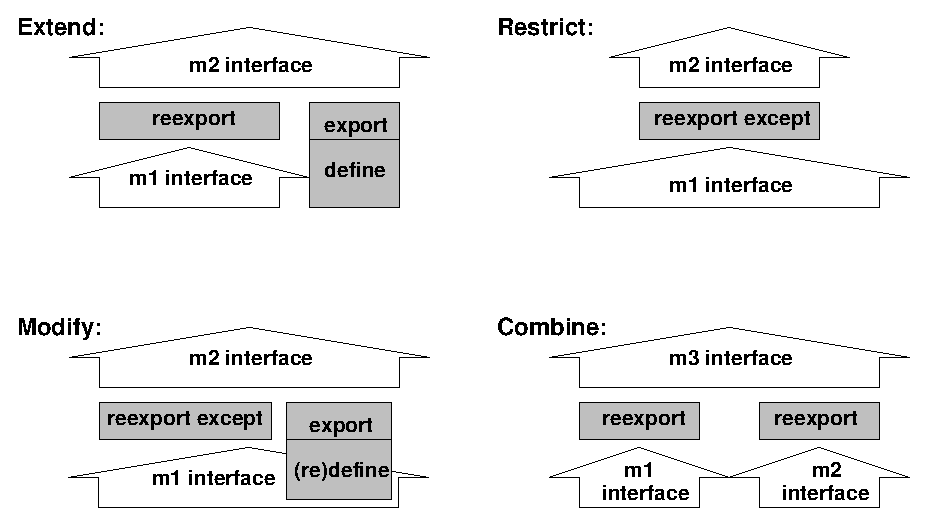
\includegraphics{reexport.eps}
\end{center}
\caption{Making modules from modules with reexport}
\label{reexport}
\end{figure}


%----------------------------------------------------------------------
\subsection{Modules and Source Files}
\index{source files}
%----------------------------------------------------------------------

When a source file contains no module directives, it becomes part of
the module from which its compilation was invoked.  This makes it
possible to write small programs without caring about modules. 
However, serious applications should be structured into modules. 

Often it is the most appropriate to have one file per module and to
have the file name match the module name.

It is however possible to have several modules in one file, e.g.\ a
main module and one or more auxiliary modules - in that
case the name of the main module should match the filename.
Every module-directive in the file marks the end of the previous
module and the start of the next one.

It is also possible to spread the contents of a module over several
files. In this case, there should be a main file whose filename
matches the module name, and the other files should be referenced
from the main file using the \bipref{include/1}{../bips/kernel/directives/include-1.html} directive, e.g.
\begin{quote}\begin{verbatim}
:- module(bigmodule).
:- include(part1).
:- include(part2).
\end{verbatim}\end{quote}



%----------------------------------------------------------------------
\subsection{Tools and Caller Modules}
%----------------------------------------------------------------------

\subsubsection{Tools}
\index{Tools}
\index{procedure!tool}
\label{tools}
There are predicates in a modular system that need to know from which
module they were called (since this may be different from the module
in which they were defined).
\index{meta-predicates}
The most common case is where a predicate is a meta-predicate,
i.e.\ a predicate that has another goal or predicate name as an argument.
Other cases are I/O predicates - they need to be executed in a
certain module context in order to obey the correct syntax of this module.
In {\eclipse}, such predicates that need to know their caller module
are called {\bf tool} predicates\footnote{
    Many Prolog systems call them meta-predicates.}.

Tool predicates must be declared.  As a consequence, the system will
automatically add a {\bf caller module} argument whenever such a tool
predicate is called.

Consider for example a predicate that calls another predicate twice.
\index{twice/1}
The naive version of this predicate looks like
\begin{quote} \begin{verbatim}
twice(Goal) :-
    call(Goal),
    call(Goal).
\end{verbatim} \end{quote}
As long as no modules are involved, this works fine.
Now consider the situation where the definition of twice/1 and a
call of twice/1 are in two different modules:
\begin{quote} \begin{verbatim}
:- module(stuff).
:- export twice/1.
twice(Goal) :-
    call(Goal),
    call(Goal).

:- module(main).
:- import stuff.

top :- twice(hello).

hello :- writeln(hi).
\end{verbatim} \end{quote}
This will not work because hello/0 is only visible in module main
and an attempt to call it from within twice/1 in module stuff will
raise an error. The solution is to declare twice/1 as a tool and
change the code as follows:
\begin{quote} \begin{verbatim}
:- module(stuff).
:- export twice/1.
:- tool(twice/1, twice/2).
twice(Goal, Module) :-
    call(Goal)@Module,
    call(Goal)@Module.
\end{verbatim} \end{quote}
What happens now is that the call to twice/1 in module main
\begin{quote} \begin{verbatim}
..., twice(hello), ...
\end{verbatim} \end{quote}
is effectively replaced by the system with a call to twice/2 where
the additional argument is the module in which the call occurs:
\begin{quote} \begin{verbatim}
..., twice(hello, main), ...
\end{verbatim} \end{quote}
This caller module is then used by twice/2 to execute
\begin{quote} \begin{verbatim}
..., call(hello)@main, ...
\end{verbatim} \end{quote}
The 
\biprefnoidx{call(Goal)@Module}{../bips/kernel/control/A-2.html}
\index{\atsym/2} construct means that the call is supposed to happen
{\em in the context} of module main.


The debugger trace shows what happens:
\begin{quote} \begin{verbatim}
[main 5]: top.
  (1) 1 CALL  top
  (2) 2 CALL  twice(hello)
  (3) 3 CALL  twice(hello, main)
  (4) 4 CALL  call(hello) @ main
  (5) 5 CALL  call(hello)
  (6) 6 CALL  hello
S (7) 7 CALL  writeln(hi)
hi
S (7) 7 EXIT  writeln(hi)
  (6) 6 EXIT  hello
  ...
\end{verbatim} \end{quote}

One complication that can arise when you use tools is that the compiler
must know that a predicate is a tool in order to properly compile
a call to the tool.
If the call occurs textually before the tool
declaration,  this will therefore give rise to an
{\bf inconsistent tool redefinition} error.
The
\bipref{tool/2}{../bips/kernel/modules/tool-2.html}
declaration must therefore occur before any call to the tool.


\subsubsection{System Tools}
\index{tool!system}
Many of the system built-in predicates are in fact tools, e.g.
\bipref{read/1}{../bips/kernel/ioterm/read-1.html},
\bipref{write/1}{../bips/kernel/ioterm/write-1.html},
\bipref{record/2}{../bips/kernel/record/record-2.html},
\bipref{compile/1}{../bips/kernel/database/compile-1.html}, etc.
All predicates which handle modular items must be tools
so that they know from which module they have been called.
In case that the built-in predicate has to be executed in
a different module (this is very often the case inside
user tool predicates), the 
\biptxtref{@ /2}{\atsym /2}{../bips/kernel/control/A-2.html}
construct must be used, e.g.
\begin{quote}\begin{verbatim}
current_predicate(P) @ SomeModule
\end{verbatim}\end{quote}


%----------------------------------------------------------------------
\subsection{Lookup Module vs Caller Module}
\index{lookup module}
\index{caller module}
%----------------------------------------------------------------------

The following table summarises the different call patterns with and
without module specifications.
There are only two basic rules to remember:
\begin{itemize}
\item \bipref{: /2}{../bips/kernel/control/N-2.html}
	specifies the {\bf lookup module} (to find the definition)
\item \biprefnoidx{@ /2}{../bips/kernel/control/A-2.html}
% need a separate index entry because latex evaluates \atsym too early
% inside \bipref
\index{\atsym/2} 
	specifies the {\bf caller module} (to know the context)
\end{itemize}

\begin{tabular}{|p{5cm}|p{4cm}|p{4cm}|}
\hline
Call inside module(m)	& Module where definition of twice/1 is looked up
	    & Caller module argument added to twice/1 \\
\hline
..., twice(X), ...		&  m &  m \\
..., lm : twice(X), ...		& lm &  m \\
..., twice(X) @ cm, ...		&  m & cm \\
..., lm : twice(X) @ cm, ...	& lm & cm \\
..., call(twice(X)) @ cm, ...	& cm & cm \\
\hline
\end{tabular}


%----------------------------------------------------------------------
\subsection{The Module Interface}
%----------------------------------------------------------------------
The primitive 
\bipref{current_module/1}{../bips/kernel/modules/current_module-1.html}
can be used to check for the existence of a module, or to enumerate
all currently defined modules.

Further details about existing modules can be retrieved using
\index{properties!module}
\bipref{get_module_info/3}{../bips/kernel/modules/get_module_info-3.html},
in particular information about the module's interface, what other
modules it uses and whether it is locked (see~\ref{locking}).


%----------------------------------------------------------------------
\subsection{Module-related Predicate Properties}
%----------------------------------------------------------------------
Information about a predicate's properties can be retrieved using the 
\index{properties!predicate}
\bipref{get_flag/3}{../bips/kernel/database/get_flag-3.html} primitive
or printed using \bipref{pred/1}{../bips/kernel/env/pred-1.html}.
The module-related predicate properties are
\begin{description}
\item[defined]
	(on/off) indicates whether code for the predicate has already
	been compiled. If not, only a declaration was encountered.
\item[definition_module]
	(an atom) the module where the predicate is defined.
\item[visibility]
	(local/exported/reexported/imported) indicates the visibility
	of the predicate in the caller module.
\item[tool]
	(on/off) indicates whether the predicate has been declared a tool.
\end{description}
For tool predicates, 
\bipref{tool_body/3}{../bips/kernel/modules/tool_body-3.html}
can be used to retrieve the predicate it maps to when the module
argument is added.

To get information about a predicate visible in a different module,
use for instance
\begin{quote}\begin{verbatim}
    get_flag(p/3, visibility, V) @ othermodule
\end{verbatim}\end{quote}

%----------------------------------------------------------------------
\section{Less Common Topics}
%----------------------------------------------------------------------

%----------------------------------------------------------------------
\subsection{Modules Using Other Languages}
%----------------------------------------------------------------------

Modules created with the \bipref{module/1}{../bips/kernel/modules/module-1.html} directive automatically import
\index{language}
\index{eclipse_language}
the module {\tt eclipse_language},  which provides the standard set
of {\eclipse} built-in predicates. 
To create a module that uses a different language dialect, use
\bipref{module/3}{../bips/kernel/modules/module-3.html}.
For instance
\begin{quote}\begin{verbatim}
:- module(mystdcode, [], iso).
\end{verbatim}\end{quote}
creates a module in which you can use ISO Standard Prolog\footnote{to the
extent implemented by {\eclipse}'s compatibility library},
but not all of {\eclipse}'s usual language features.
Note that the third argument (here {\tt iso}) simply
specifies a library which implements the desired language,
so new languages can be added easily.


%----------------------------------------------------------------------
\subsection{Creating and Erasing Modules at Runtime}
%----------------------------------------------------------------------
\begin{sloppypar}
A module can also be created explicitly by a running program with
\bipref{create_module/1}{../bips/kernel/modules/create_module-1.html} or
\bipref{create_module/3}{../bips/kernel/modules/create_module-3.html}
and erased with
\bipref{erase_module/1}{../bips/kernel/modules/erase_module-1.html}. 
The latter should be used with care, erasing a module while a
predicate defined in that module is being executed can provoke
unpredictable results. The same holds for trying to erase essential
system modules.
\end{sloppypar}


%----------------------------------------------------------------------
\subsection{Initialization and Finalization}
\label{initfini}
\index{initialization}
\index{finalization}
%----------------------------------------------------------------------
Sometimes modules have global state which needs to be initialised
or finalised. For this purpose, modules can have
\begin{description}
\item[Local Initialization Goals:]
these are specified as
\begin{quote}\begin{verbatim}
:- local initialization(Goal).
\end{verbatim}\end{quote}
and are executed just after the module containing them has been loaded.
\item[Exported Initialization Goals:]
these are specified as
\begin{quote}\begin{verbatim}
:- export initialization(Goal).
\end{verbatim}\end{quote}
and are executed whenever the module containing the declaration gets
imported into another module. The call will happen in the context of
the importing module.
\item[Finalization Goals:]
these are specified as
\begin{quote}\begin{verbatim}
:- local finalization(Goal).
\end{verbatim}\end{quote}
and are executed just before the module containing them gets erased.
Modules can get erased either explicitly through
\bipref{erase_module/1}{../bips/kernel/modules/erase_module-1.html} 
or implicitly when the module is re-compiled, or when the {\eclipse}
session is exited.  Finalization goals should not do any I/O because
in the case of an embedded ECLiPSe, I/O may no longer be available at
finalization time.

\end{description}

%----------------------------------------------------------------------
\subsection{Locking Modules}
\label{locking}
\index{locking}
%----------------------------------------------------------------------
By default, {\eclipse} does not strictly enforce the hiding of
module internals. This facilitates program development as is makes
it possible to inspect and trace without being too concerned about module
boundaries. E.g.\ you can set a spy point on a local predicate p/3
in module othermod by calling:
\begin{quote}\begin{verbatim}
:- spy(p/3)@othermod.
\end{verbatim}\end{quote}
Once a module implementation is stable and there is a need for privacy,
it is possible to {\em lock} a module. Locking makes it impossible
to access internal, local items from outside the module. Of course,
the module can still be used though its interface.
The built-in predicates related to locking are
\bipref{lock/0}{../bips/kernel/modules/lock-0.html} which provides
a definitive lock,
\bipref{lock_pass/1}{../bips/kernel/modules/lock_pass-1.html}
which allows subsequent unlocking using a password (
\bipref{unlock/2}{../bips/kernel/modules/unlock-2.html}),
and
\bipref{get_module_info/3}{../bips/kernel/modules/get_module_info-3.html}
which allows to check whether a module is locked.
\bipref{lock/0}{../bips/kernel/modules/lock-0.html} and
\bipref{lock_pass/1}{../bips/kernel/modules/lock_pass-1.html} are
usually used as a directive in the source file of the module to be locked.

%HEVEA\cutend
